\documentclass[tikz,border=5pt]{standalone}
\usepackage{ctex,amsmath}
\usetikzlibrary{arrows.meta,calc}
\tikzset{>=Latex,orbit/.style={gray!70,thick},
 pvec/.style={blue!70!black,very thick,->},
 fvec/.style={orange!85!black,very thick,->},
 guide/.style={gray!60,dashed}}
\begin{document}
\begin{tikzpicture}[font=\large]
 \draw[orbit](0,0)circle(2.1);
 \draw[guide](-2.1,0)--(2.1,0);
 \fill(0,0)circle(.035)node[above]{$O$};
 \fill[red!75!black](2.1,0)circle(.07);
 \fill[blue!70!black](-2.1,0)circle(.07);
 \node[above right]at(2.35,.25){$+Ze,\ m_0$};
 \node[above left]at(-2.35,.25){$-Ze,\ m_0$};
 \draw[pvec](2.1,.10)--(2.1,1.35)node[right]{$\boldsymbol v_+$};
 \draw[pvec](-2.1,-.10)--(-2.1,-1.35)node[left]{$\boldsymbol v_-$};
 \draw[fvec](2.0,0)--(.9,0)node[midway,below]{$F$};
 \draw[fvec](-2.0,0)--(-.9,0)node[midway,below]{$F$};
 \draw[guide](-2.1,-.12)--(-2.1,-3.2);
 \draw[guide](2.1,-.12)--(2.1,-3.2);
 \draw[guide](0,-.12)--(0,-2.62);
 \draw[<->](-2.1,-2.55)--(0,-2.55)node[midway,above]{$r_0/2$};
 \draw[<->](0,-2.55)--(2.1,-2.55)node[midway,above]{$r_0/2$};
 \draw[<->](-2.1,-3.15)--(2.1,-3.15)node[midway,below]{$r_0$};
 \node[gray!70!black]at(0,2.72){轨道平面俯视};
\end{tikzpicture}
\begin{tikzpicture}[font=\large]
 \begin{scope}
  \draw[orbit](0,0)circle(1.35);
  \fill(0,0)circle(.025)node[above]{$O$};
  \fill(0,-1.35)circle(.045);
  \draw[pvec](0,-1.35)--(1.2,-1.35)node[below]{$\boldsymbol p(t)$};
  \draw[fvec](0,-1.25)--(0,-.25)node[right]{$\boldsymbol F$};
  \node at(0,2.0){位置空间};
  \draw[<->](-.25,0)--(-.25,-1.35)node[midway,left]{$\rho$};
 \end{scope}
 \begin{scope}[xshift=5.8cm]
  \draw[orbit](0,0)circle(1.75);
  \coordinate(P)at(1.75,0);
  \coordinate(Q)at({1.75*cos(32)},{1.75*sin(32)});
  \fill(0,0)circle(.025)node[below left]{$O_p$};
  \draw[pvec](0,0)--(P);
  \draw[pvec](0,0)--(Q);
  \node[right]at(1.82,-.2){$\boldsymbol p(t)$};
  \node[above right]at(Q){$\boldsymbol p(t+\Delta t)$};
  \draw[fvec](P)--(Q)node[midway,right]{$\Delta\boldsymbol p$};
  \draw[->](.6,0)arc[start angle=0,end angle=32,radius=.6];
  \node at(.4,.9){$\Delta\varphi$};
  \node at(0,2.4){动量空间};
  \node at(1.4,-2.35){$|\Delta\boldsymbol p|=2p\sin(\Delta\varphi/2)$};
 \end{scope}
\end{tikzpicture}
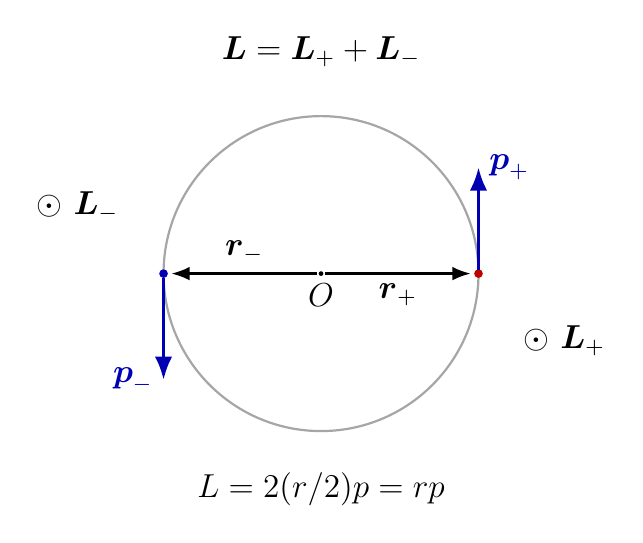
\begin{tikzpicture}[font=\large]
 \draw[orbit](0,0)circle(2.0);
 \fill(0,0)circle(.03)node[below]{$O$};
 \draw[->,thick](.05,0)--(1.9,0)node[midway,below]{$\boldsymbol r_+$};
 \draw[->,thick](-.05,0)--(-1.9,0)node[midway,above]{$\boldsymbol r_-$};
 \fill[red!75!black](2,0)circle(.055);
 \fill[blue!70!black](-2,0)circle(.055);
 \draw[pvec](2,.05)--(2,1.35)node[right]{$\boldsymbol p_+$};
 \draw[pvec](-2,-.05)--(-2,-1.35)node[left]{$\boldsymbol p_-$};
 \node[right]at(2.45,-.85){$\odot\ \boldsymbol L_+$};
 \node[left]at(-2.45,.85){$\odot\ \boldsymbol L_-$};
 \node[above]at(0,2.5){$\boldsymbol L=\boldsymbol L_++\boldsymbol L_-$};
 \node[below]at(0,-2.4){$L=2(r/2)p=rp$};
\end{tikzpicture}
\begin{tikzpicture}[font=\large,x=6cm,y=3.5cm]
 \fill[red!7](1,0)rectangle(1.3,1.18);
 \draw[->](-.03,0)--(1.36,0)node[right]{$\beta$};
 \draw[->](0,-.03)--(0,1.24)node[above]{$r/r_{\mathrm{NR}}$};
 \draw[blue!70!black,very thick,domain=.008:.9998,samples=160]
  plot(\x,{sqrt(1-\x*\x)});
 \draw[guide](0,.8)--(.6,.8)--(.6,0);
 \fill[blue!70!black](.6,.8)circle(.01);
 \draw[guide](1,0)--(1,1.16);
 \draw[fill=white,draw=blue!70!black,line width=.8pt](0,1)circle[radius=3pt];
 \draw[fill=white,draw=blue!70!black,line width=.8pt](1,0)circle[radius=3pt];
 \node[left]at(0,1){$1$};
 \node[left]at(0,.8){$0.8$};
 \node[below]at(.6,0){$0.6$};
 \node[below]at(1,0){$1$};
 \node[blue!70!black]at(.38,.45){$\sqrt{1-\beta^2}$};
 \node[align=center]at(1.16,.8){无正半径\\圆轨道};
 \node[gray!70!black,above right]at(.02,1.04){弱耦合极限};
 \node at(.63,-.29){$\beta=\alpha Z^2/(2n),\qquad r_{\mathrm{NR}}=2n^2\hbar^2/(m_0A)$};
\end{tikzpicture}
\begin{tikzpicture}[font=\large,x=1cm,y=1cm]
 \begin{scope}
  \clip(.12,-1.5)rectangle(6.5,4.4);
  \draw[blue!70!black,very thick,domain=.13:6.4,samples=200]
   plot(\x,{2*sqrt(1+1/(\x*\x))-1.2/\x});
  \draw[orange!85!black,thick,domain=.13:6.4,samples=200]
   plot(\x,{2*sqrt(1+1/(\x*\x))-2/\x});
  \draw[red!70!black,thick,domain=.13:6.4,samples=200]
   plot(\x,{2*sqrt(1+1/(\x*\x))-2.4/\x});
 \end{scope}
 \draw[->](0,0)--(6.7,0)node[right]{$x$};
 \draw[->](0,-1.55)--(0,4.55)node[above]{$H/(m_0c^2)$};
 \draw[guide](0,2)--(6.5,2);
 \node[left]at(0,2){$2$};
 \node[left]at(0,0){$0$};
 \draw[guide](4/3,0)--(4/3,1.6);
 \fill[blue!70!black](4/3,1.6)circle(.055);
 \node[below]at(4/3,0){$x_*$};
 \node[blue!70!black,right]at(7.0,3.65){$A/(cL)=1.2$};
 \node[orange!85!black,right]at(7.0,3.05){$A/(cL)=2$};
 \node[red!70!black,right]at(7.0,2.45){$A/(cL)=2.4$};
 \node[gray!70!black,right]at(7.0,1.45){$x=m_0cr/L$};
 \node[right]at(7.0,.55){固定总角动量$L$};
\end{tikzpicture}
\end{document}
